\documentclass[11pt]{article}

\usepackage{fullpage}
\usepackage{amsmath}
\usepackage{epsfig}
\usepackage{graphics}
\usepackage{caption}
\usepackage{circuitikz}

\oddsidemargin -0.15in
\evensidemargin -0.15in
\headheight 0in
\headsep 0in
%\topmargin -0.25in
\textheight 9.3in
\textwidth 6.8in
\captionsetup{width=0.9\textwidth} 

\begin{document}


\begin{center}
\section*{
Franklin \& Marshall College \hfill PHY 223\\
\bigskip
{\Large \it BB Scattering}}
\end{center}
 
In any scattering experiment, a projectile flies toward a target and is scattered. The scattering interaction
may be a physical collision (e.g., for two billiard balls) or another force (e.g., a Coulomb repulsion or gravitational attraction). Over the course of many such scattering events, the
scattering pattern (i.e., the directions of all scattered particles) is recorded
in some manner. Finally, the scattering pattern is analyzed in order to give
some information about the shape of the target and its interactions with the projectiles. The information
provided by a scattering experiment is indirect and incomplete, but it is often
the only information we can get about objects we want to study.

Two of the important variables used in scattering discussions are illustrated in
Fig. \ref{fig: b parameter}. The incoming particles have various values of $b$,
the \textbf{impact parameter}, which measures their perpendicular distance from the
central axis when they are traveling toward the target. After scattering, the particles travel outward with a \textbf{scattering angle} $\theta$, which is the change in angle from their initial velocity. The value of $b$ and the strength of the interaction force jointly
determine the scattering angle $\theta$.

\vspace{3mm}

\noindent \noindent \begin{minipage}{\linewidth}
  \centering
  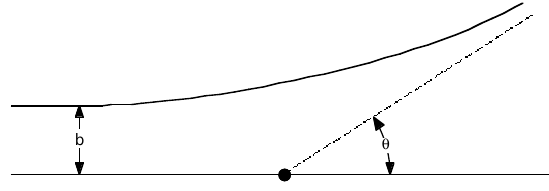
\includegraphics[scale=2.3]{b_parameter.png}
  \captionof{figure}{A particle coming in from the left with impact parameter
    $b$ scatters at angle $\theta$.}
  \label{fig: b parameter}
\end{minipage}

\vspace{3mm}

In a real scattering experiment, we do not launch particles individually at specific values of $b$. 
Instead, we have an incoming ``beam'' of many particles that each have different (and typically random) 
values of $b$ spread over the area of the beam, each of which will scatter with a different angle $\theta$.
Some, generally smaller, values of $b$ result in large scattering angles; while
other, generally larger, values of $b$ lead to small scattering angles. This is
illustrated in Fig. \ref{fig: db dtheta}. There is some area perpendicular to the
beam, labeled $\Delta\sigma$ in Fig. \ref{fig: db dtheta}, that results in
scattering into the angular range $\Delta\theta$. This $\Delta\sigma$ is the \textbf{cross section} for scattering into $\Delta\theta$. For 3D experiment, $\Delta\sigma$ has units of area because any particles of the beam that pass through that area will have a scattering angle between $\theta$ and $\theta+\Delta\theta$

\vspace{3mm}

\noindent \begin{minipage}{\linewidth}
  \centering
  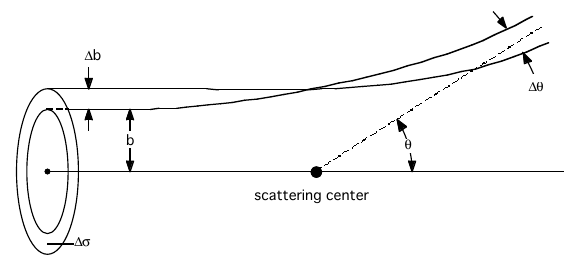
\includegraphics[scale=2.3]{db_dtheta.png}
  \captionof{figure}{All incoming particles incident on the cross sectional area
  $\Delta\sigma$ are scattered into the angular range $\Delta\theta$.}
  \label{fig: db dtheta}
\end{minipage}

\vspace{3mm}

The beam intensity is described by the \textbf{flux} $\Phi$, which is the number of beam
particles per unit area per unit time. That is, if the beam has a cross
sectional area of $A$, the total rate of beam particles per second is $r=\Phi A$. If we want to know
the rate at which particles will scatter into our specific range of angles $\Delta \theta$, we should
instead multiply the flux by the corresponding cross sectional area $\Delta \sigma$:
% Thus the product of the flux times the scattering cross section gives the rate
% $\Delta r$ for particles to scatter into angular range $\Delta\theta$:

\begin{equation}
\Delta r = \Phi \Delta\sigma
\end{equation}

\noindent where $\Delta r$ describes the number of particles per second that have a scattering angle in the range $\Delta \theta$. If we consider a large $\Delta \theta$ (i.e., a large range of scattering angles) we should expect to capture a large fraction of the total scattered particles. Therefore, we can also write the equation above explicitly in terms of how $\Delta r$ relates to $\Delta \theta$:

\begin{equation}
\Delta r = \Phi \frac{d\sigma}{d\theta}\Delta \theta
\end{equation}

% \noindent which displays the proportionality between $\Delta r$ and
% $\Delta\theta$. We have used the differential relationship $\Delta\sigma =
% (d\sigma/d\theta) \Delta\theta$, where $d\sigma /d\theta$ is known as the
% ``differential cross section'' of the target. Of course, if there is more than one
% target particle (as is usually the case for atomic or nuclear targets), the
% expressions for $\Delta r$ must be multiplied by the number of targets.

\noindent where have used the differential relationship $\Delta\sigma =
(d\sigma/d\theta) \Delta\theta$, and $d\sigma /d\theta$ is known as the
\textbf{differential cross section} of the target.

Here we can see that the rate $\Delta r$ is
proportional to $\Delta \theta$, but that this rate also depends on the relationship
 between $\sigma$ and $\theta$. If there is only a small area of the target that will cause a 
 specific scattering angle, then we will have fewer particles scattering with that angle. The differential
 cross section is therefore determined by the physics of the interactions between the incoming
 particle and the target (i.e., the shape and orientation of the target and the types 
 of forces involved).
 Of course, if there is more than one
target particle (as is usually the case for atomic or nuclear targets), the
expressions for $\Delta r$ must be multiplied by the number of targets, but we will consider 
a single target here.


In our experiment, we will also simplify things by making all of the motion occur in
 a horizontal plane (i.e., in 2D rather than 3D). Consequently,
the cross section for scattering into a given angular range $\Delta\theta$ is
really a cross sectional \textit{length}, not a cross sectional \textit{area}. Likewise, 
our beam is really a band of particles spread over a width $h$ instead of an area $A$ 
(see Fig. \ref{fig: flux}), so the intensity of our beam will be based on the 
number of particles per unit length rather than per area. Finally, for 
purposes of this experiment we remove the ``per unit time'' part of
the flux definition since we will be launching our particles one by one and counting them up
at the end, rather than having a continuous flow.  Based on these simplifications, we will 
redefine our ``flux'' as $\Phi=n/h$: the number of particles $n$ that we launch, divided by
the length $h$ over which they are spread.

As you think about this particle ``beam'', it is important to remember that the flux of a beam
(whether in 3D or 2D) is determined completely by the properties of the beam and is independent
of the particular target that happens to be present. We could imagine putting targets of 
different shapes and sizes into the same beam and getting different distributions of scattering angles,
but the flux $\Phi$ of the beam describes the \textit{incoming} distribution of particles before they interact 
with the target.

\vspace{3mm}

\noindent \begin{minipage}{\linewidth}
  \centering
  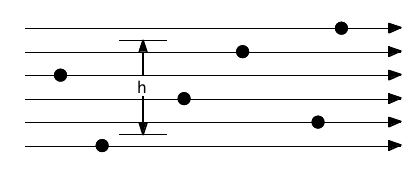
\includegraphics[scale=2.3]{flux.png}
  \captionof{figure}{In our experiment the beam of particles is a horizontal
    band. The beam strength is measured by a ``flux'' $\Phi = n/h$ equal to the
    ratio of $n$, the number of particles, to the length $h$ measured 
    perpendicular to the beam.}
  \label{fig: flux}
\end{minipage}

\vspace{3mm}

The target in this experiment is a circular disk of radius $R$, which we can use to find
the scattering angle $\theta$ as a function of $b$ and then
the differential cross section $d\sigma/d\theta$ for scattering off of this
target.
%(see Fig. \ref{fig: scattering}).
We start with the law of reflection, which states that the incident angle
equals the final angle (both measured with respect to the normal). The geometry
of this scattering is shown in Fig. \ref{fig: scattering mech}.

\vspace{3mm}

\noindent \begin{minipage}{\linewidth}
  \centering
  % 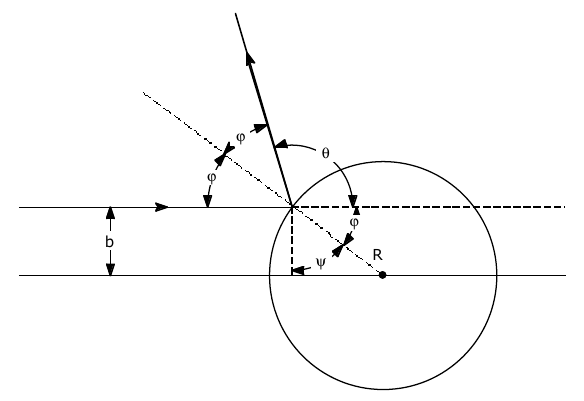
\includegraphics[scale=2.5]{scattering_mech.png}
  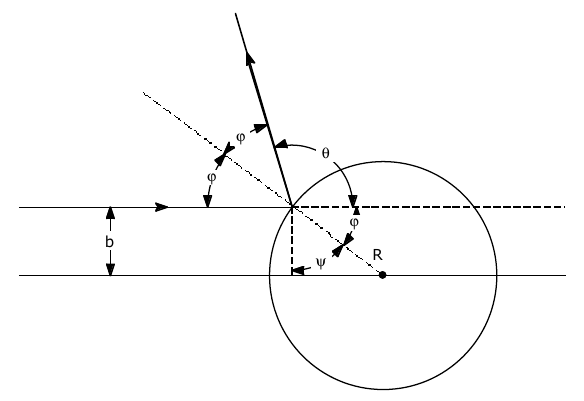
\includegraphics[scale=2.3]{scattering_mech.png}
  \captionof{figure}{The geometry for a BB of impact parameter $b$ scattering
    off of a disk of radius $R$. The scattering angle between the initial and
    final direction is $\theta$.}
  \label{fig: scattering mech}
\end{minipage}

\vspace{3mm}


From the
trigonometry of right triangles, one has $\cos(\psi) = b/R$, so that $\psi =
\cos^{-1}(b/r)$. From Fig.~\ref{fig: scattering mech} we can see that $\phi = \pi/2 - \psi$ , so
that 
$\theta = \pi - 2\phi = 2\psi = 2\cos^{-1}(b/R)$ and therefore:
% \begin{equation}
% \[
% \theta = \pi - 2\phi = 2\psi = 2\cos^{-1}(b/R)\,,\qquad\textrm{and therefore}
% \]
% \end{equation}
% \noindent It follows that
\begin{equation}
b = R\cos(\theta/2)
\label{eq:b(theta)}
\end{equation}

% \noindent which is the desired relation between $b$ and $\theta$. 
Now that we know the scattering
angle at each particular value of $b$, we can determine the differential cross section by considering
how a range of $b$ values (i.e., particles with impact parameters between $b$ and $b+\Delta b$) will
scatter into a range of angles between $\theta$ and $\theta+\Delta \theta$ as shown in Fig.~\ref{fig: scattering}:

\vspace{3mm}

\noindent \begin{minipage}{\linewidth}
  \centering
  % 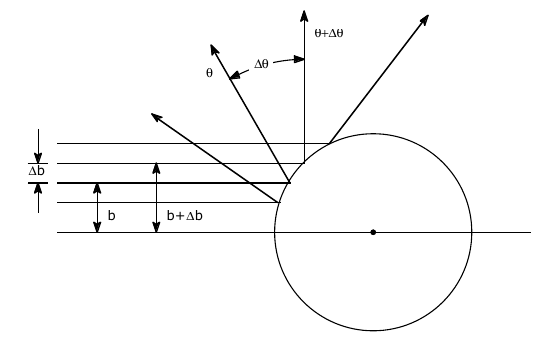
\includegraphics[scale=2.5]{scattering.png}
  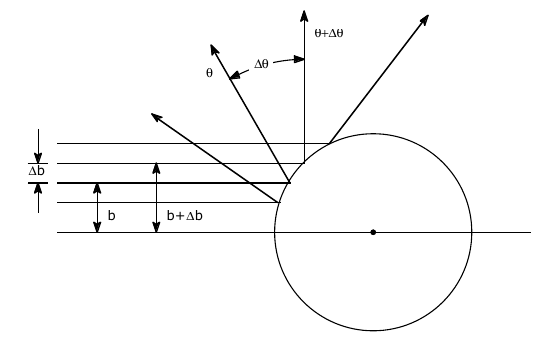
\includegraphics[scale=2.3]{scattering.png}
  \captionof{figure}{All particles with impact parameter between $b$ and
    $b+\Delta b$ will be scattered with angle between $\theta$ and
    $\theta+\Delta\theta$. The cross sectional length $\Delta\sigma =
    (d\sigma/d\theta) \Delta\theta$ is just equal to $\Delta b$.}
  \label{fig: scattering}
\end{minipage}

\vspace{3mm}

\noindent Specifically, 
% the range of $b$ values that will scatter within a range of $\theta$ values, whic
the impact
parameter that corresponds to scattering at angle $\theta+\Delta \theta$ is:

\begin{eqnarray}
  b' &=& b+\Delta b \\
    %  &=& R\cos\left( \frac{\theta+\Delta \theta}{s} \right) \\
     &=& b+\frac{db}{d\theta}\Delta \theta \\
     &=& R\cos\left( \frac{\theta}{2} \right) + R\left[ \frac{d}{d\theta}\cos\left(
      \frac{\theta}{2} \right) \right]\Delta \theta \\
     &=& R\cos\left( \frac{\theta}{2} \right)-\frac{R}{2}\sin\left(
         \frac{\theta}{2} \right) \Delta \theta
\end{eqnarray}

\noindent Thus the range in $b$ that results in scattering at angles between
$\theta$ and $\theta+\Delta\theta$ is

\begin{equation}
\Delta b = b'-b = -\frac{R}{2}\sin\left( \frac{\theta}{2} \right)\Delta \theta
\end{equation}

\noindent where the minus sign reflects the fact that a larger $b$ gives a smaller
$\theta$. Now the cross
sectional length $\Delta \sigma$ for these scattering angle is just range of impact parameters that produces that range of angles:

\begin{equation}
  \Delta \sigma = \frac{d\sigma}{d\theta}\Delta\theta=|\Delta b| = \frac{R}{2}
  \sin\left( \frac{\theta}{2} \right) \Delta\theta
\end{equation}

\noindent Note we have used $|\Delta b$| because the cross section is a positive value (regardless of direction). Consequently, the differential cross section is

\begin{equation}
\frac{d\sigma}{d\theta} = \frac{R}{2}\sin\left( \frac{\theta}{2} \right)
\end{equation}

\noindent The final result for the number of particles $N$ scattered into
angular range $\Delta \theta$ at scattering angle $\theta$ is

\begin{equation}
N = \Phi\frac{R}{2}\sin\left( \frac{\theta}{2} \right) \Delta \theta
\end{equation}

\vspace{5mm}

\noindent {\bf Experimental setup}

You will shoot a large number of BBs through a hand operated BB gun at a rigid
circular target. Data will be recorded as dots on pressure sensitive tape
attached to the circular ``particle detector'' surrounding and concentric with the
target. You will analyze this data to determine the radius of the target.

You will use the Welsh BB gun and scattering apparatus with a round plastic
target attached, a number of BBs, a meter stick, calipers, masking tape, and a
length (about 1.1m) of pressure sensitive tape.

\vspace{5mm}

\noindent {\bf Procedures}

\begin{enumerate}

\item Turn the position setting screw so that the BBs just miss the target.
Shoot a few BBs for practice.

\item Use masking tape to affix the pressure sensitive tape (with the white side
showing) to the inside surface of the detector. By left-right symmetry, it is
sufficient to study the scattering off of one side of the target instead of
both. So, cover only half of the detector with pressure sensitive tape—starting
at the gun opening and going in the same direction as the gun's displacement.

\item Shoot five BBs. Turn the position setting screw one-half revolution so
that the gun points closer to the target and shoot five more BBs. Continue to
shoot five BBs per half revolution until the BBs are bouncing back at the gun.
Do not try to keep track of which mark on the tape was produced by which BB in
the beam. (This kind of information would not be available in an actual
scattering experiment.)

\item Remove the pressure sensitive tape for analysis.

\item Find the ``flux'' $\Phi$ for your beam. Remember that the ``flux'' is the number of particles
fired per unit length (see Fig. 3). It can be found as follows:

  \begin{enumerate}
  \item Figure how many particles were fired while the positioning screw was
    rotated 10 times. Call this number $n$.
  \item Measure the length of the range of positions over which these $n$ particles were fired.
    Call this distance $h$.
  \item The ``flux'' is then $\Phi = n/h$.
  \end{enumerate}
  
\item Locate the $\theta = 0$ point on your tape (see Fig. \ref{fig: bins}). This
is where the BBs just barely miss the target (and so are not scattered). Mark
``bins'' on your tape starting 1 cm past the $\theta = 0$ point. Make sure each bin
 has the same width and that you make a note of the bin width you choose, which should 
 be about 5cm. Label them as bin 1, bin 2, etc. starting from the bin
closest to $\theta=0$, and count how many particles $N_i$ scattered into the
i$^{th}$ bin for $i=1, 2, \ldots$ etc.
  

  \vspace{3mm}

  \noindent \begin{minipage}{\linewidth}
    \centering
    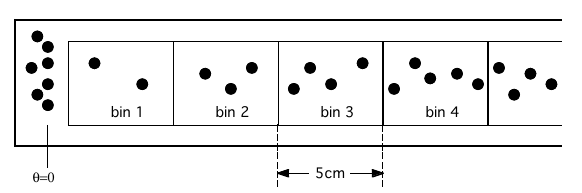
\includegraphics[scale=2.5]{bins.png}
    \captionof{figure}{Your data tape will look something like this. The
      rightmost edge of the accumulation of dots to the left occurs at
      $\theta=0$. The angle $\theta_i$ of the i$^{th}$ bin is found by measuring the
      distance between the $\theta=0$ point and the center of the bin, and then
      dividing by the detector radius.}
    \label{fig: bins}
  \end{minipage}
  \vspace{3mm}

  \item You now have the data that you will use to analyze the scattering from this experiment! As part of that analysis, you will eventually need to convert the position measurements on your data tape to angles using the relation $\theta=s/R_D$ , where $s$ is the arc length along the edge of the detector corresponding to the angle to be measured, and $R_D$ is the radius of the detector. With this in mind, make sure to measure and record the radius of your detector to use in your analysis.
\end{enumerate}

\end{document}
